%                            ================================
%                            [Type doctument]
%                            - \documentclass[option]{class}
%                            [Other page setup]
%                            - geometry: set margin, should
%                                similar with \documentclass
%                            ================================
\documentclass[12pt, a4paper, twoside]{report}
\usepackage[a4paper,inner=3cm,outer=2cm, top=2cm, bottom=2.5cm]{geometry}

%============================================================
% Preamble
% - Include packages allow expand ability of Texlive by more 
%       commands, environments
% - Commands effect entire document
%============================================================
%                            ================================
%                            Package
%                            - lipsum: lorem paragraph
%                            Url
%                            - hyperref: url
%                            Color
%                            - color, xcolor
%                            Language format
%                            - inputenc, fontenc, babel
%                            - lmodern: Latin modern
%                            Table
%                            - array: format tabular row
%                            - graphicx: table size
%                            Render basic
%                            - rotating: rotate object 
%                                       (static or float)
%                            - rotfloat: addition float rotating
%                            - float: addition H absolute position
%                               for rotfloat or table, figure evironment
%                            - graphicx: image like PNG, IMG, PDF
%                            Mathematic
%                            - mathtools: include amsmath
%                            - amssymb: expand math symbols
%                            Sourcecode:
%                            - listings
%                            Abbreviations table
%                            - nomencl : make nomenclature table
%                            Glossary part
%                            - glossaries
%                            Index part
%                            - makeidx
%                            - \makeindex
%                            ================================
\usepackage{lipsum}
\usepackage[hidelinks]{hyperref}
% \usepackage{color}
\usepackage[table]{xcolor}

\usepackage[utf8]{inputenc}
\usepackage[T1, T5]{fontenc}
\usepackage{lmodern} % a Latin font version enhance from
                        % cm-supper + vector format + better support T1,T5
\usepackage[english, vietnamese]{babel} 


\usepackage{array}
\usepackage{graphicx}


\usepackage{rotating}
\usepackage{rotfloat}

\usepackage{float}

\usepackage{graphicx}

\usepackage{mathtools}
\usepackage{amssymb}

\usepackage{listings}


\usepackage{nomencl}
\makenomenclature
\renewcommand{\nomname}{List of Abbreviations}

\usepackage{glossaries}
\makeglossaries

\usepackage{makeidx}
\makeindex
%============================================================
% Document
% - Plain text, list of tables, figures, input other tex, 
%       bibilography, ...
% - Commands with scope: in group
% - Environments differ from 'document': 
%       /begin{env} , /end{env}
%============================================================
\begin{document}

%                                                        ================================
%                                                        [Pre define]
%                                                        1. Glossary definitions(help build)
%                                                        2. Page setup
%                                                        ================================


%                            ================================
%                            Glossary definitions (help build)
%                            ================================
% Define glossary before use refer by gls{}


\newglossaryentry{lorem 1}
{
    name=lorem paragraph 1,
    description=
    {is a part of template document issued from package `lipsum'.\\
    Paragraph number: 1}
}

\newglossaryentry{lorem 2}
{
    name=lorem paragraph 2,
    description=
    {is a part of template document issued from package `lipsum'.\\
    Paragraph number: 2}
}

\newglossaryentry{computer}
{
    name=computer,
    description=
    {is a programmable machine that receives input,
    stores and manipulates data, and provides
    output in a useful format}
}

%                            ================================
%                            Page setup
%                            - pagestyle: set header, footer
%                            ================================
\pagestyle{headings}



%                                                        ================================
%                                                        [Front matter]
%                                                        1. Title page
%                                                        2. Empty
%                                                        3. Information (copyright notice, ISBN, etc.)
%                                                        4. Dedication, Acknowledgements if any, else empty
%                                                        5. Table of contents
%                                                        6. Abbreviations  
%                                                        7. LOT, LOF
%                                                        8. Preface chapter
%                                                        9. Abstract 
%                                                        ================================


%                            ================================
%                            Title
%                            ================================
\title
{
    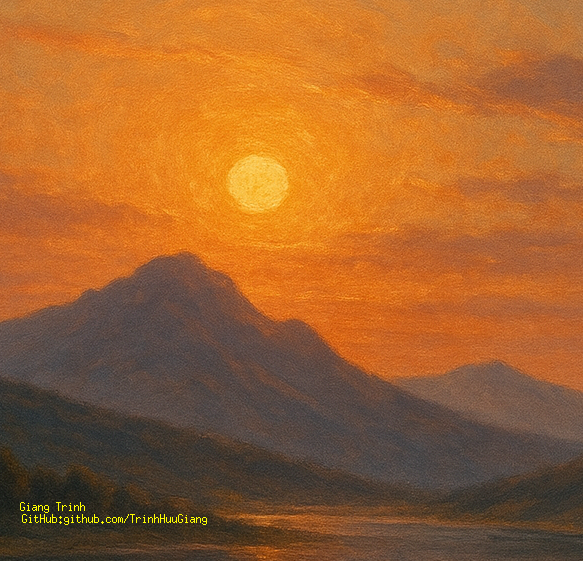
\includegraphics[width=5cm]{./sunset.png} \\
    \textbf{Hello\thanks{\LaTeX {} wikibook}}
}
\author{Giang Trinh\thanks{GitHub: \url{{https://github.com/TrinhHuuGiang}}}
    \and others\thanks{No one}}
\maketitle

%                            ================================
%                            Table of contents
%                            - TOC, LOF, LOT
%                            ================================
% \tableofcontents
\printnomenclature
% \listoftables
% \listoffigures


%                            ================================
%                            Abstract
%                            ================================


%                                                        ================================
%                                                        [Main matter]
%                                                        Main topics
%                                                        ================================



%                            ================================
%                            Main topic
%                            ================================
\chapter{This is test chapter}

\gls{lorem 1}
\nomenclature[group 1]{Lorem 1}{Lorem paragraph 1}
\index{Lorem 1}
Lorem ipsum dolor sit amet, consectetuer adipiscing elit. Ut purus elit, vestibulum ut,
placerat ac, adipiscing vitae, felis. Curabitur dictum gravida mauris. Nam arcu libero,
nonummy eget, consectetuer id, vulputate a, magna. Donec vehicula augue eu neque.
Pellentesque habitant morbi tristique senectus et netus et malesuada fames ac turpis
egestas. Mauris ut leo. Cras viverra metus rhoncus sem. Nulla et lectus vestibulum urna
fringilla ultrices. Phasellus eu tellus sit amet tortor gravida placerat. Integer sapien est,
iaculis in, pretium quis, viverra ac, nunc. Praesent eget sem vel leo ultrices bibendum.
Aenean faucibus. Morbi dolor nulla, malesuada eu, pulvinar at, mollis ac, nulla. Curabitur
auctor semper nulla. Donec varius orci eget risus. Duis nibh mi, congue eu, accumsan
eleifend, sagittis quis, diam. Duis eget orci sit amet orci dignissim rutrum.\\

\gls{lorem 2}
\nomenclature[group 1]{Lorem 2}{Lorem paragraph 2}
\index{Lorem 2}
Nam dui ligula, fringilla a, euismod sodales, sollicitudin vel, wisi. Morbi auctor lorem
non justo. Nam lacus libero, pretium at, lobortis vitae, ultricies et, tellus. Donec aliquet,
tortor sed accumsan bibendum, erat ligula aliquet magna, vitae ornare odio metus a mi.
Morbi ac orci et nisl hendrerit mollis. Suspendisse ut massa. Cras nec ante. Pellentesque
a nulla. Cum sociis natoque penatibus et magnis dis parturient montes, nascetur ridiculus
mus. Aliquam tincidunt urna. Nulla ullamcorper vestibulum turpis. Pellentesque cursus
luctus mauris.\\


\newpage

\gls{lorem 1}
\nomenclature[group 2]{Lorem 1}{Lorem paragraph 1}
\index{Lorem 1}
Lorem ipsum dolor sit amet, consectetuer adipiscing elit. Ut purus elit, vestibulum ut,
placerat ac, adipiscing vitae, felis. Curabitur dictum gravida mauris. Nam arcu libero,
nonummy eget, consectetuer id, vulputate a, magna. Donec vehicula augue eu neque.
Pellentesque habitant morbi tristique senectus et netus et malesuada fames ac turpis
egestas. Mauris ut leo. Cras viverra metus rhoncus sem. Nulla et lectus vestibulum urna
fringilla ultrices. Phasellus eu tellus sit amet tortor gravida placerat. Integer sapien est,
iaculis in, pretium quis, viverra ac, nunc. Praesent eget sem vel leo ultrices bibendum.
Aenean faucibus. Morbi dolor nulla, malesuada eu, pulvinar at, mollis ac, nulla. Curabitur
auctor semper nulla. Donec varius orci eget risus. Duis nibh mi, congue eu, accumsan
eleifend, sagittis quis, diam. Duis eget orci sit amet orci dignissim rutrum.\\

\gls{computer}

%                                                        ================================
%                                                        Back matter
%                                                        - Appendix
%                                                        - Glossary
%                                                        - Bibliography
%                                                        - Index
%                                                        ================================


%                            ================================
%                            Appendix
%                            - Subordinate chapters
%                            - More explanations
%                            ================================



% Glossary
\printglossaries


% indexing
\printindex




%                            ================================
%                            END
%                            ================================
\end{document}

